%%%%%%%%%%%%%%%%%%%%%%%%%%%%%%%%%%%%%%%%%%%%%%%%%%%%%%%%%%%%%%%%%%%%%
%%%
%%% Set these variables appropriately
%%%
\newcommand{\AUTHORS}{Ravi Tandon, Haoyu Zhang \\ Guide: Prof. Kai Li \\ COS 598D \\ Analytics and Systems of Big Data \\}
\newcommand{\TITLE}{What can go wrong with in-memory computation frameworks}
\newcommand{\KEYWORDS}{}
\newcommand{\CONFERENCE}{}
\newcommand{\PAGENUMBERS}{yes}       % "yes" or "no"
\newcommand{\TOAPPEAR}{no}
%%%
%%%
%%%%%%%%%%%%%%%%%%%%%%%%%%%%%%%%%%%%%%%%%%%%%%%%%%%%%%%%%%%%%%%%%%%%%

%%%% Setup the document/page
\documentclass[pdftex,twoside,twocolumn,10pt,letterpaper]{article}
\usepackage{ifthen}

\ifthenelse{\equal{\PAGENUMBERS}{yes}}{%
\usepackage[nohead,
            left=1in,right=1in,top=1in,
            footskip=0.5in,bottom=0.75in     % Room for page numbers
            ]{geometry}
}{%
\usepackage[noheadfoot,columnsep=0.2in,
            margin=1in,centering,truedimen]{geometry}
}

\usepackage{fancyhdr}
\usepackage{floatrow}
\usepackage[numbers,sort]{natbib}
\usepackage{xspace}
\usepackage{booktabs}
\usepackage{subfigure}
\usepackage[T1]{fontenc}
\usepackage{textcomp}
\usepackage{mathptmx}   % Times + Times-like math symbols
\usepackage{courier}
\usepackage[scaled=0.92]{helvet}
\usepackage[scaled=.8]{beramono}

\usepackage{color}
\usepackage[pdftex]{graphicx}
\ifthenelse{\isundefined{\wantBW}}{%
  \usepackage[colorlinks]{hyperref}%        % for online version
}{%
  \usepackage[pdfborder={0 0 0}]{hyperref}% % for paper (B&W) version
}
\newcommand{\URL}[1]{\url{#1}}

%%%%% Setup for PDF
\hypersetup{%
pdfauthor = {\AUTHORS},
pdftitle = {\TITLE},
pdfsubject = {\CONFERENCE},
pdfkeywords = {\KEYWORDS},
bookmarksopen = {true}
}
\usepackage{titlesec}
\titlespacing\section{0pt}{12pt plus 4pt minus 2pt}{0pt plus 2pt minus 2pt}
%\setlength{\parindent}{0pt}
%\setlength{\parskip}{0pt}
\renewcommand{\headrulewidth}{0pt}
\newcommand{\Paragraph}[1]{\vspace{-2ex}\paragraph{#1.}}
\setlength{\topmargin}{-.14in}

\ifthenelse{\equal{\PAGENUMBERS}{yes}}{%
  \pagestyle{plain}
}{%
  \pagestyle{empty}
}

\makeatletter\long\def\@makecaption#1#2{
   \vskip 10pt
   \setbox\@tempboxa\hbox{\textsf{#1: #2}}
   \ifdim \wd\@tempboxa >\hsize % IF longer than one line:
       \textsf{#1: #2}\par      % THEN set as ordinary paragraph.
     \else                      % ELSE  center.
       \hbox to\hsize{\hfil\box\@tempboxa\hfil}
   \fi}
\makeatother

\clubpenalty=10000  % Don't allow orphans
\widowpenalty=10000 % Don't allow widows

\title{\textbf{\TITLE}}
\author{\AUTHORS}
\date{}

% Compact itemize and enumerate.  Note that they use the same counters and
% symbols as the usual itemize and enumerate environments.
\def\compactify{\itemsep=0pt \topsep=0pt \partopsep=0pt \parsep=0pt}
\let\latexusecounter=\usecounter
\newenvironment{CompactItemize}
  {\def\usecounter{\compactify\latexusecounter}
   \begin{itemize}}
  {\end{itemize}\let\usecounter=\latexusecounter}
\newenvironment{CompactEnumerate}
  {\def\usecounter{\compactify\latexusecounter}
   \begin{enumerate}}
  {\end{enumerate}\let\usecounter=\latexusecounter}

\newcommand{\comment}[1]{\textcolor{red}{#1}}
\newcommand{\ignore}[1]{}

\newcommand{\xc}[1]{\mbox{\textit{#1}}}
\newcommand{\la}{\leftarrow}
\newcommand{\ra}{\rightarrow}
\newcommand{\somespace}{\hspace{0.1cm}}

\def\discretionaryslash{\discretionary{/}{}{/}}
\def\discretionarydot{\discretionary{.}{}{.}}
\def\discretionarycolon{\discretionary{:}{}{:}}
{\catcode`\/\active
\catcode`\.\active
\catcode`\:\active
\gdef\URLprepare{\catcode`\/\active\let/\discretionaryslash
                 \catcode`\.\active\let.\discretionarydot
                 \catcode`\:\active\let:\discretionarycolon
        \def~{\char`\~}}}%
\def\URL{\bgroup\URLprepare\realURL}%
\def\realURL#1{\tt #1\egroup}%

\newcommand{\eg}{{\em e.g.}, }
\newcommand{\ie}{{\em i.e.}, }
\newcommand{\etal}{{\em et al.\ }}

\def\check{\stackrel{{\scriptscriptstyle ?}}{=}}

\begin{document}
\maketitle

% -*-LaTeX-*-
% $Id: abstract.tex 70 2007-01-30 21:59:16Z nicolosi $

\begin{abstract}
Whislt the advent of in-memory computation platforms for big-data
applications has considerably improved application throughput, it has
also significantly increased the reliance on the available memory
resources within individual computing nodes.  The current design of
large scale data computation platforms makes use of commodity servers,
which typically have limited resources on each node.  In this paper we
present an analysis of the impact of this tension that could possibly
hamper future big-data computing platforms.  To reveal the effects of
memory pressure on big-data applications running on Spark, we conduct
experiments to quantify the impact of garbage collection done by storage
management on the application throughput. Besides, we present results
based on object level access patterns of an application running on Spark
through a unique interception mechanism oblivious to applications.
Additionally, we extend the abstraction of RDDs by providing indexing
capabilities within key-valued RDDs. We show that simple range
partitioning of real world log data can help reduce query time when
using RDDs. 
\end{abstract}

   
\section{Introduction} 
\label{sec:intro}
\paragraph{}
With the advent of big data systems such as \cite{zaharia2012resilient, engle2012shark, agarwal2013blinkdb} large computations have been pushed within memory of the computing nodes. While reduction in the dependence on secondary storage for fault-tolerance can improve the performance throughput significantly, it increases the memory pressure on the application. Our belief is that as systems scale, memory would become a bottleneck for applications that rely heavily on memory. We, therefore, investigate the effect of memory pressure on a state of the art runtime engine (\textit{Spark}) and point out the fundamental issues in extending current systems owing to specific access patterns of these applications. Additionally, we suggest extensions in the design of RDDs that can significantly reduce in-memory computation, thus lending to better scalability. 
\paragraph{}
Spark is an in-memory runtime that supports large big data workloads. Spark introduces the concept of \textit{Resilient Distributed Datasets (RDDs)} which are large data sets and can be partitioned across several nodes. RDDs use a global namespace and therefore are globally visible from every node within the cluster. Internally, Spark, models computations as graphs of tasks much like \textit{Dryad} \cite{isard2007dryad} and computes lineages based these computation graph models for resilience. Inherently, Spark pushes computations and the corresponding data in memory, unlike the MapReduce \cite{dean2008mapreduce} framework that relies on intermediate persistence for fault tolerance. We posit that such frameworks will be bottlenecked by the available DRAMs as the applications scale. We identify two basic reasons for this. Firstly, commodity servers typically run with 4GB or 8GB of RAM and therefore processing data on the order of hundreds of gigabytes of data can require tens of server machines. This could not only increase the cost of the cluster, it would result in heavy overheads due to excessive network and disk bandwidth utilization. Scaling DRAM is not a viable option since the cost of DRAM (\$/GB) goes exponentially higher as DRAM sizes increase beyond 64GB. \cite{badam2011ssdalloc} Secondly, runtimes such as Spark are built on managed runtimes such as Scala. Scala runs on top of Java Virtual Machine (JVM). JVM increases the overall overhead and results in significant reduction in application throughput due to memory management overheads. \cite{yang2006cramm}
\paragraph{}
	We therefore investigate the performance of a big data application over 5 different configurations and show that applications that use in-memory computation frameworks would perform better if memory per node can scale well. Horizontal scaling supports larger workloads at the cost of a reduction in the application throughput due to increased communication costs. In order to develop deeper insight into possible solutions to scale applications we have designed a unique interception mechanism within the Java Virtual Machine that profiles an application’s access patterns at the object level. We observe that applications have a heavy tailed access pattern which can be exploited to extend  memory management systems to better scale applications by transparently and dynamically profiling the workload.  In order to reduce computation and communication costs, we propose generic extensions to RDDs by range partitioning them. We refer to these RDDs as IRDDs \textit{(Indexed RDDs)}. We find such range partitioning schemes to be useful for running filtering queries on log based datasets.
\paragraph{}
	The rest of the paper is organized as follows. Section \ref{sec:motivation} provides higher level ideas that motivated this work. Section \ref{sec:design} describes the design of our work.  Section \ref{sec:implementation} discusses implementation details of I-RDDs. Section \ref{sec: related} describes some of the related work. Section \ref{sec:experiments} describes our evaluation. Section \ref{sec:conclusion} provides a brief summary of our work.

\section{Motivation} 
\label{sec:motivation}
\paragraph{}
With the advent of Spark like Big data runtimes big data, workloads will create excessive pressure on the current memory subsystems. We believe that current memory subsystems are not well suited to handle spikes of memory requirement and will get severely affected by non-uniform memory requirement patterns. Fig \ref{fig:fig1} shows the overall time it takes for the Garbage Collector for different tasks when running a page ranking application. The initial tasks require a large amount of memory. We believe this could be because of the extra memory required when reading data from the secondary storage (due to deserialization of data). There is a subsequent drop in the throughput for these specific set of tasks. This was the primary motivation for studying the effect of memory pressure on different configurations. Besides, we believe, the answer to better memory management lies in understanding the underlying access patterns of different workloads and offloading low priority data on hybrid memory subsystems. Therefore, we performed experiments quantifying access patterns in baseline spark system.

\begin{figure}[!ht]
\caption{Overall time spent in garbage collection for tasks with 2GB and 6GB of memory per node}
\label{fig:fig1}
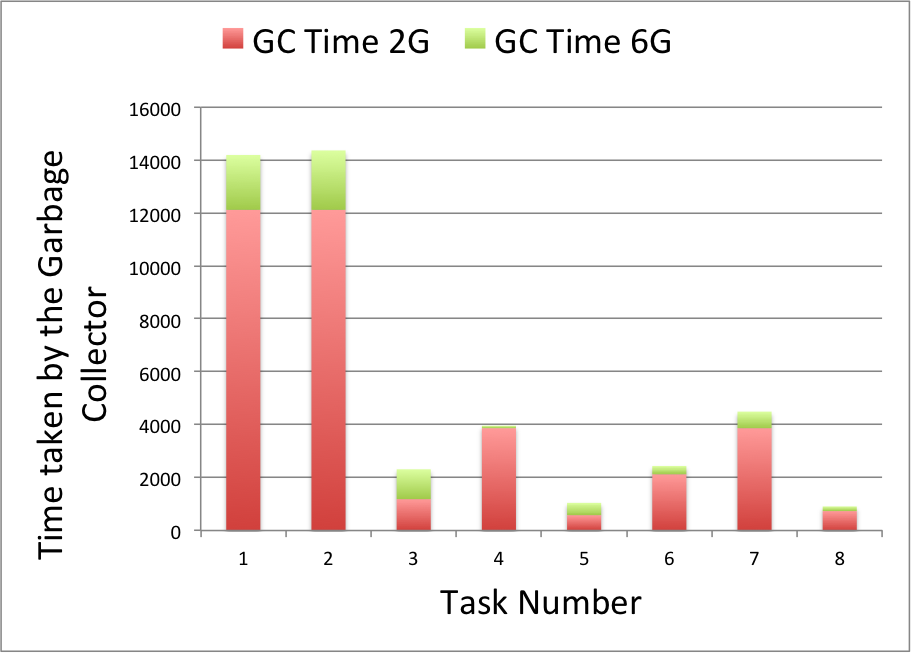
\includegraphics[scale=0.50]{./images/image1.png}
\end{figure}

\paragraph{}
	Another, observation we had is that the abstraction of RDDs is still inept when handling search queries on semi-structured datasets such as logs from applications, page views etc. When filtering a dataset Spark has to parse all the partitions within a dataset, while the actual results might be contained in a subset of the overall partitions. Fig \ref{fig:fig2} shows the comparison between Vanilla Spark's filtering query and an ideal implementation of a set of queries on a dump from Wikimedia \cite{wikimedia} where we observe that on an average only 48\% of the total partitions contained relevant results. This was the primary motivation behind building a range partitioning mechanism on top of partitions and thereby indexing the data stored in RDDs.

\begin{figure}[!ht]
\caption{Comparison of query runtimes on Vanilla (V-Spark) and an ideal query engine (I-Spark)}
\label{fig:fig2}
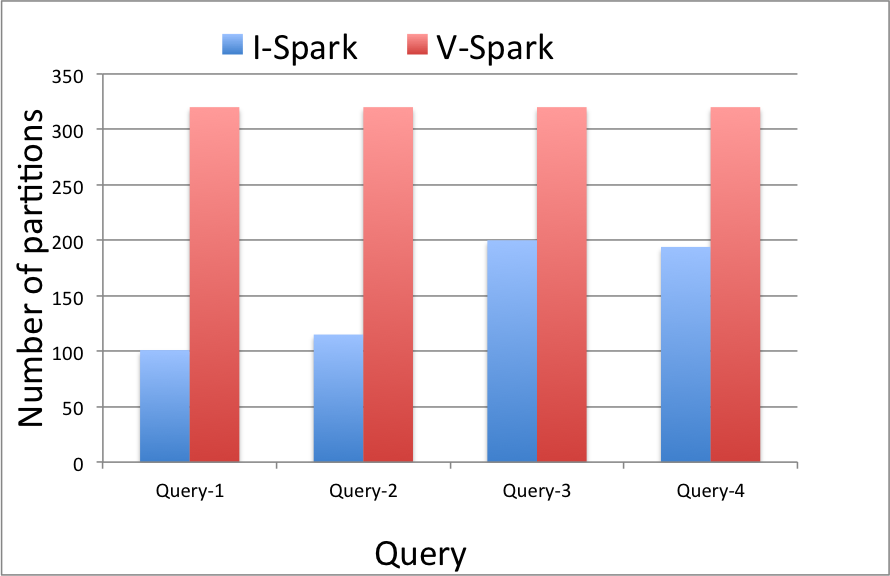
\includegraphics[scale=0.50]{./images/image2.png}
\end{figure}


\section{Design} 
\label{sec:design}
We first describe the basic design of Spark. Spark abstracts data in the
form of a globally addressable data structure called Resilient
Distributed Dataset. The RDD is divided into smaller partitions, each of
which is an array of the unit (the unit is the class type of data).  In
order to execute a job on Spark, a driver program requests the master
node to schedule a given task on the worker nodes. The job (in our case
a filter query) is then executed in four basic steps: 
\begin{enumerate}
\item The master node requests file metadata from the underlying Hadoop
    file system. A lazy read on the file is performed, meaning the data
    is read into the memory only when an action has to be performed on
    the RDD. Based on the file metadata, the master node computes the
    appropriate partitions on the file size. (Spark uses a maximum size
    of \emph{33MB} per partition). 
\item The master then sends the \texttt{jar} file containing the job to
    the different worker nodes along with the set of partitions on which
    each of the worker node has to perform the job. 
\item The worker nodes read the data from the distributed file system
    into their local memory. Thereafter, they execute the actions on the
    RDDs and return the result back to the master node.
\item The master node then performs necessary completion actions on the
    job (generally an aggregation of the results) and returns the result
    back to the driver.
\end{enumerate}

\paragraph{Index Creation:}
In our design, the driver program initially requests the creation of an
index on the RDD given a specific key.  The Spark runtime sends a job
(for index creation) to each of the worker node, which then reads the
allocated partition and computes a pair of keys.  This pair denotes the
smallest and the largest keys within the partition and essentially is
the range of the partition.  The master then retrieves the range for
each partition and then aggregates them into a single in-memory array.
Any subsequent queries on the specified key are performed through a
different sequence of steps.

For any lookup query on the key, the master node computes the partitions
which include the key within their range. The master node then runs the
job on the filtered set of RDDs which may contain the key. The job is
then sent to the different worker nodes. Each of the worker node
performs the job on their respective of partitions and returns the
result back to the master. The master then aggregates the result and
sends it back to the driver. 

\paragraph{Design of Indexed RDDs:}
We support indexing on top for RDDs wherein each record can be
structured as a key-value pair.  We range-partition the RDDs. For each
partition the highest and lowest key (according to an appropriate class
comparison function) is computed.  This is thereafter stored as the
metadata for each partition, and later on used for any subsequent
queries to compute the possible subset of partitions within which the
keys can exist and the corresponding query is run on the RDD. In our
current design, the range partitioning is done by the master and cached
in memory, as a map of partition index as the
key and range as the corresponding value.

In addition to the support for range partitioning, we also support a
fast indexing scheme if the key-value structured data is sorted on the
key. The indexer stores the smallest value for each partition and caches
it in memory. Since the keys are sorted, any subsequent pair of keys can
be used as a range for the preceding partition. Thereafter, the master
can efficiently figure out the range of partitions within which a
querying key would fall in. 

\paragraph{Design of JVM prototype:}
For our virtual machine prototype, we use an open source Java Virtual
Machine, \emph{Oracle's OpenJDK framework} \cite{openjdk}. A Java
program is compiled into an intermediate bytecode representation. Object
accesses are compiled into \texttt{load} and \texttt{store}
instructions. We intercept these instructions and put in extra
instructions to increment the counter of an object on each access.  JVM
abstracts each Java object as a class instance within the virtual
machine.  In order to achieve a low overhead on each object access, we
add an extra field within the object header and increment the counter on
every object access. This allows us to monitor accesses on each object
throughout the Java program's execution.


\section{Implementation} 
\label{sec:implementation}
\paragraph{}
We here describe the implementation of our indexed RDDs. We create a separate derived class IndexedRDDKV, with the RDD class as its base class. We support the following interfaces on the RDD class:
\begin{enumerate}
\item \textit{indexedKV():} The driver program can call indexedKV() on any RDD to transform the given RDD into an RDD of key, values which supports indexing. Each record must be a key-value pair. 
We expose the following interfaces on the IndexedRDDKV class:
\item \textit{rangePartitions ():} The method creates a range partitioned index on the data in the RDDs. For each partition, the smallest and the largest value is stored as the range of the partition.
\item \textit{searchByKeyRangePartitioned (key: String):} This method searches for the key within the range partitions. The master first filters the set of partitions within which the key can exist and then runs the query on those select partitions. 
\item \textit{indexPartitions():} The indexPartitions method is used to create a partition on the range of keys when the input data is already sorted. 
\item \textit{searchByKey(key: String):} The search by key function searches the given string within the RDD using the index created by the indexedPartitions function. 
\end{enumerate}
\section{Evaluation}
\label{sec:eval}

\subsection{Study of the effect of garbage collection on Spark runtime}
\paragraph{}
Our first set of experiments were conducted to understand the effect of
memory pressure on applications by quantifying the impact of garbage
collection when running a PageRank application on Spark. The high level
questions that we wanted to answer are as follows:

\begin{enumerate}
\item What is a good strategy of scaling big-data applications? (more
    cores, less memory per core versus less cores, more memory per core) 
\item What is the impact of managed runtimes on application throughput?
\item What is the more fundamental problem with the way memory is managed
    by runtime engines when running big-data applications on Spark?
\end{enumerate}

\paragraph{Experimental Setup:}
The experiments were conducted on machines with Intel Xeon processors
running at clock frequency of 2.66GHz, with 4 cores per processor, and
16 GB of DRAM. Each machine runs Linux version 2.6.18 with L1 cache
size of 32K.

\paragraph{Experimental 1:}
The experiments are conducted on the following five different configurations:
\begin{itemize}
\item Configuration 1 (15W, 1G): The configuration consists of 15 worker nodes, each with 1 GB of memory.
\item Configuration 2 (10W, 1G): The configuration consists of 10 worker nodes, each with 1 GB of memory.
\item Configuration 3 (5W, 2G):  The configuration consists of 5 worker nodes, each with 2 GB of memory.
\item Configuration 4 (2W, 5G):  The configuration consists of 2 worker nodes, each with 5 GB of memory.
\item Configuration 5 (1W, 7.5G):The configuration consists of 1 worker node, each with 7.5 GB of memory.
\end{itemize}

\paragraph{}
The application we run is the vanilla PageRanking algorithm provided
with the Spark library. The dataset that we take describes a network
which was collected by crawling Amazon website. It is based on the
\textit{Customers Who Bought This Item Also Bought} feature of the
Amazon website. If a product $i$ is frequently co-purchased with product
$j$, the graph contains a directed edge $i \rightarrow j$
\cite{leskovec}. It includes a graph of \textit{403394 nodes} with
\textit{3387388 nodes}. The data is around \textit{50MB} in size. The
page ranking algorithm was run for \textit{10 iterations}.

Table \ref{tab:table1} lists out the running times, along with the
overheads due to the garbage collector for different configurations.

\begin{table}[h!]
\begin{tabular}{| c | c | c | c |}
\hline
Configuration  & Application Run  &  \% Overhead  \\ 
& Time (in ms) & due to GC \\ \hline
15W, 1G & 428,245  & 33\% \\ \hline
10W, 1G & 414,742 &  30.5\% \\ \hline
5W, 2G & 216,320 & 23\%  \\ \hline
2W, 5G & 152159 & 15.29\% \\ \hline
1W, 7.5G & 164893 & 8.45\% \\ \hline
\end{tabular}
\caption{Comparison of the overhead in throughput due to garbage collection for different configurations}
\label{tab:table1}
\end{table}

\paragraph{Analysis of results:}
Fig. \ref{fig:exp4} shows a relative comparison of the overall
throughput from the cluster under different configuration settings. Fig.
\ref{fig:exp4_2} shows a relative comparison of the impact of garbage
collection on the cluster under these configuration settings. We can
observe that garbage collection has a detrimental effect on the overall
running time of the application. For a configuration of 2 nodes with 5
GB of memory per server, the overall running time of the application
increased by 16\%, whereas for a setup of 15 workers with 1 GB of memory
on each server the overall running time of the application was reduced
by 33\%. 

\begin{figure}[!ht]
\caption{Comparison of application runtime for different configurations}
\label{fig:exp4}
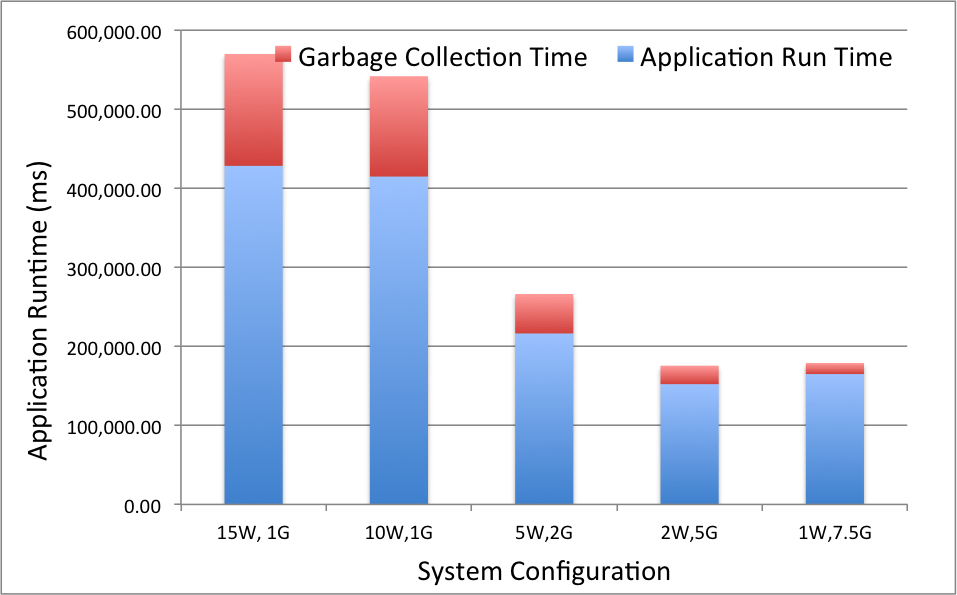
\includegraphics[scale=0.50]{./images/exp4.png}
\end{figure}

\begin{figure}[!ht]
\caption{Comparison of relative affect of garbage collection on application runtime for different configurations}
\label{fig:exp4_2}
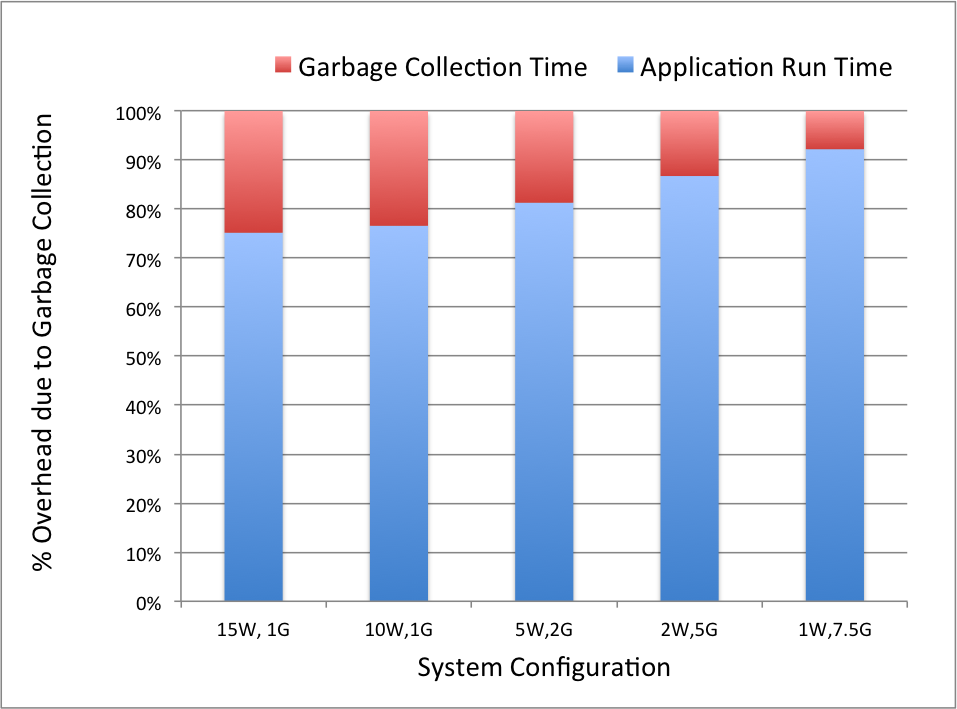
\includegraphics[scale=0.50]{./images/exp4_2.png}
\end{figure}

\begin{figure}[!ht]
\caption{Comparison of application runtime for successive tasks for two different configurations}
\label{fig:exp5}
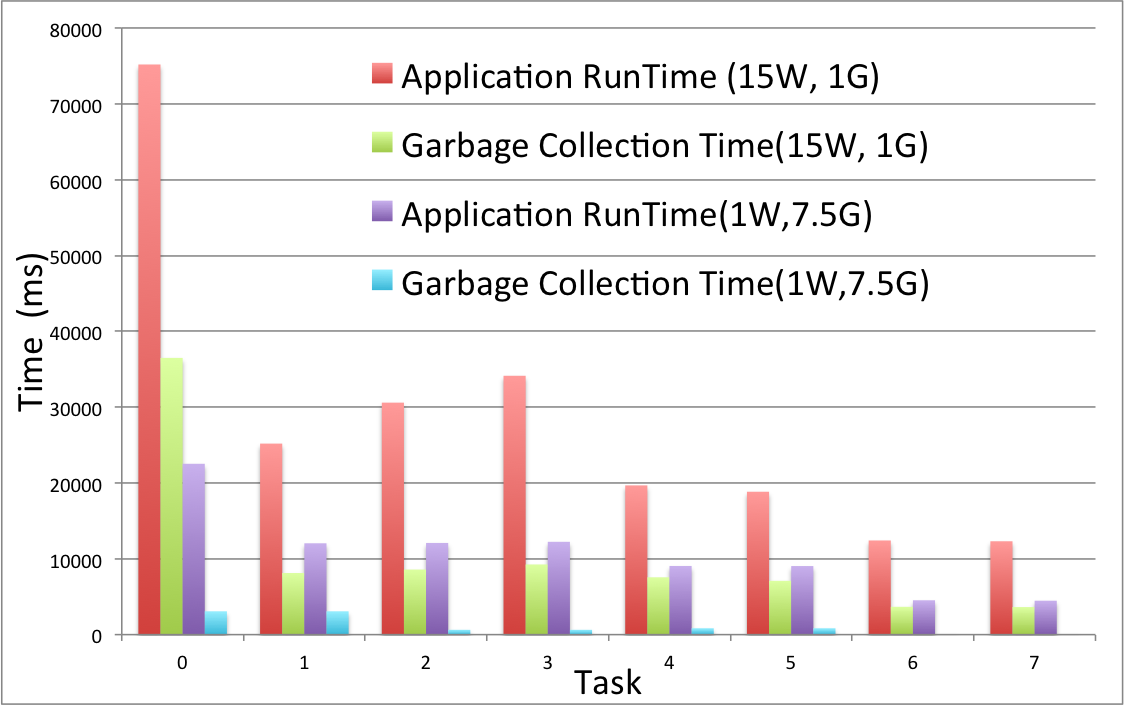
\includegraphics[scale=0.40]{./images/exp5.png}
\end{figure}

\paragraph{}
There are several reasons that explain the above behaviors.  Firstly,
Spark is an in-memory runtime application. It requires extensive amounts
of memory for storing intermediate data such as when deserializing data
read from the storage layer, maintaining cache of RDDs, lineages of RDDs
etc. Larger memory requirements creates extra memory pressure triggering
frequent garbage collection. Therefore the overall throughput of the
application decreases. Secondly, in order to scale the application, when
the number of nodes in the cluster is increased, the synchronization
costs due to communication over the network and secondary storage causes
additional overhead.  An intuitive conclusion one can derive from the
above set of experiments is that in order to scale memory-intensive
applications, horizontal scaling may not be as effective as scaling
resources on individual nodes. 

%%%%%%%%%%%%%%%%%%%%%%%%%%%%%%%%%%%%%%%%%%%%%%%%%%%%%%%%%%%

\subsection{Study of object-level access patterns within Spark} 
\paragraph{} In order to answer the second question, we took a dummy
application in Spark that calculates the value of Pi on a local machine. 

\paragraph{Objective:}
The objective of the experiment is to measure the spectrum of object
level accesses when running a baseline Spark application that does
minimal work. 

\paragraph{Experimental Setup:} 
The experiments were conducted on Intel(R) Xeon(R) CPU E3-1230 V2
machines running at a clock frequency of 3.30GHz with 8 cores with L1
cache size of 32K. For the experiment we used 512MB of memory.

\paragraph{Analysis of results:} 
The results we report are for a specific period of time for which the
application runs, since our interception mechanism (as explained in
Section \ref{sec:design}) can approximate object accesses within a
single evacuation cycle of G1 garbage collection.

Fig. \ref{fig:exp6} shows a histogram of the object-level accesses
of different component objects within the Spark application. The results
indicate a remarkable heavy-tailed object-level access pattern: within
the specified period of time, around 45,000 objects were live in the young
generation of the application; out of these, around 1,000 objects
(nearly 2\%) had an access count of over 1,000, which we labeled as
\emph{hot objects}, and contribute for nearly 58\% of the total accesses
within the survivor and eden regions.
%Nearly 17\% of the overall accesses derived from 0.02\% of the total objects.
On the other hand, nearly 3\% of the overall accesses are coming for
50\% of the objects in the specified regions of the memory.
These numbers clearly indicate that the object-level access patterns
within applications are extremely heavy-tailed. 

\begin{figure}[!ht]
\caption{Histogram of object accesses for different objects for a Spark Application}
\label{fig:exp6}
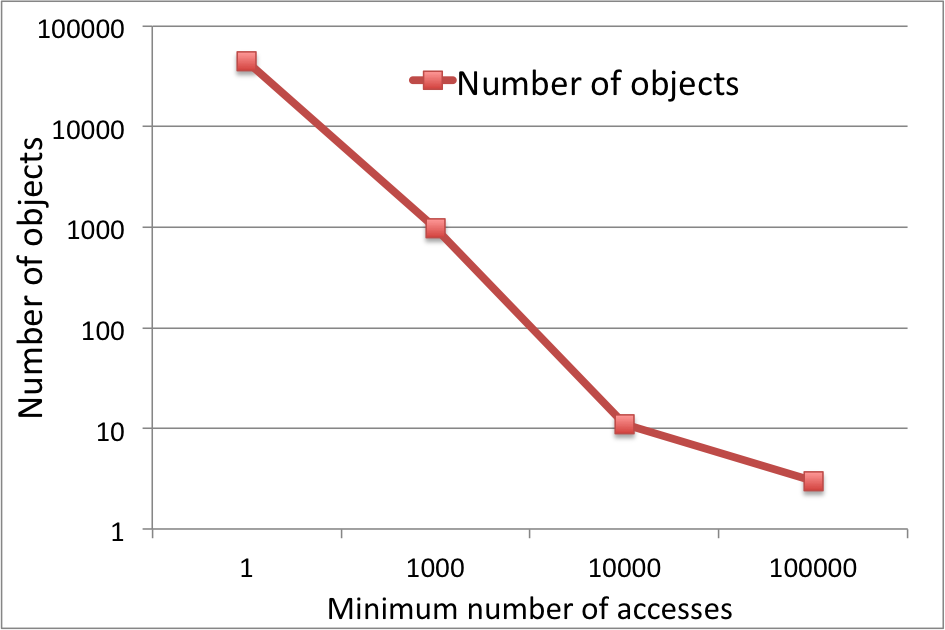
\includegraphics[scale=0.50]{./images/exp6.png}
\end{figure}

\paragraph{}
Here we give three reasons to explain the heavy tail in the distribution
of object level accesses pattern.
Firstly, accesses to large arrays of objects (such as RDDs) will have
especially high numbers since each access of an object in an array is
also an access to that array (much like a container of objects).  Such
arrays can be classified as hot objects in the object space.
Secondly, instances of objects that contain utility functions such as
methods for compressing, polling the network interfaces, DOM parsing
have large access counters. Due to their generic functionality, these
objects could become the frequent access spots.
Thirdly, a very large collection of objects (nearly half of all the
objects) such as classes for caching root names might get accessed once
and be used only at certain specific intervals, such as that at a task
start up for looking up the addresses of the different workers.  These
\emph{cold objects} show the low-usage access pattern. 
To conclude, most of the data objects likely to be frequently accessed
are arrays or utility functions (such as worker queue, XML document
handlers, symbol table entry handlers, loggers, etc.)
The objects that are less frequently
accessed are temporary objects, such as method objects, strings, classes
for caching root names, object for looking up the MIME types (used for
inspecting object headers), objects created for storing symbol tables
for compilers, parsers, etc.

\paragraph{}	
The long-tail distribution of access patterns unearths a potential
problem in contemporary memory management system design. Current virtual
memory systems have a page based abstraction for managing in-memory application
data, while data residing on the same pages might not
always have very good ``access similarity''. Paging, therefore, by virtue
of its underlying design, cannot capture the access level semantics of
applications at an appropriate granularity. This experiment provides us with
useful insights and helps further our understanding of the underlying
fundamental problems within current memory management system designs.

%%%%%%%%%%%%%%%%%%%%%%%%%%%%%%%%%%%%%%%%%%%%%%%%%%%%%%%%%%%

\subsection{Study of Indexed RDDs effectiveness}
\paragraph{Objective:} We observe that while the design of RDDs supports
caching and faster recovery through lineages, it lacks certain
capabilities. Besides, RDDs inherently support operations on datasets
which consist of pairs of key and values. We posit a natural extension
to the design of RDDs using range partitioned indexes on keys. This
experiment answers the following three questions:

\begin{enumerate}
\item How to improve the efficiency of running queries on
    semi-structured data (such as database logs, page-visit history)? 
\item What are better schemes of indexing larger datasets using RDDs?
\item How well can a generic indexing scheme based on range partitioning
    scale? 
\end{enumerate}

\paragraph{Experimental Setup:} The experiments were conducted on
machines with Intel(R) Xeon(R) CPU E3-1230 V2 running at a clock
frequency of 3.30GHz, with 8 processor cores, with 32GB of DRAM size.
Each machine runs Linux version 3.11.10 with L1 cache size of 32K.  The
experiments were run on a cluster of 3 nodes connected with 1 Gbps NICs
arranged on a single rack. The Spark setup consisted of 6 workers (2 on
each machine) and 1 master. Each of the workers was configured with 8GB
of memory and the master had 2 GB of memory.  The master physically
locates on the same machine as one of the workers. The tests were run
using using the Spark shell interface.  The experiments were conducted
on Hadoop file system (version 2.2.0).  The block size was set to
default 256MB. The Hadoop master and data nodes were set up on the same
machine.

\paragraph{Datasets:} For the experiments we used page view logs from
Wikimedia dumps \cite{wikimedia}. Wikipedia publishes page view
statistics every month.  The following is an example of the data:\\
\texttt{fr.b Special:Recherche/Achille\_Baraguey\_d\%5C\%27- Hilliers 1
624} \\
All data items are in this 4-column format. The first column
\texttt{fr.b} denotes the project name; the second column is the title
of the page retrieved; the third column is the number of requests, and
the fourth column is the size of the content returned.
In our experiments, we use the project names as the keys and the rest
parts of the lines as the values that need to be retrieved from the
underlying distributed file system.  We use two different collection of
data (10GB and 25GB), approximating 5 months and 1 years of data
respectively, with nearly 300 million and 730 million records. 

\paragraph{Experiment 3:}
For the experiments we run five different queries and measure the
overall time it takes for the queries to complete. 

Fig. \ref{fig:exp7} shows a comparison of three different configurations
when running the queries on 10GB file. VSpark denotes queries on vanilla
Spark using unindexed RDDs; ISpark\_C (Indexed Spark Coarse-Grained
Partitioned) denotes RDDs with 320 partitions; and ISpark\_F (Indexed
Spark Fine-Grained Partitioned) denotes RDDs with 1280 partitions. While VSpark
takes 87 seconds to complete, the average time for a positive query (a
query that matched keys in the file) on ISpark\_C was around 37 seconds.
Using more fine grained partitioning ISpark\_F, the average time lowers
down to 11 seconds. It is also worth noting that for queries that miss
match, the result is returned in less than one second. The reason is
that the range partitioning mechanism can pre-determine the set of RDDs
on which the query needs to be run on, which helps reduce the overall
computation that needs to done for filtering records. Besides, the
communication cost over the network also gets reduced.  For queries
result in a miss, the master can instantaneously return an empty result
by just looking up the key ranges mapping and determining that certain
key is outside the range of all the partitions.

\begin{figure}[!ht]
\caption{Comparison of query completion times between Spark, Spark Coarse-grained and Spark Fine-grained partitioned for a 10GB file}
\label{fig:exp7}
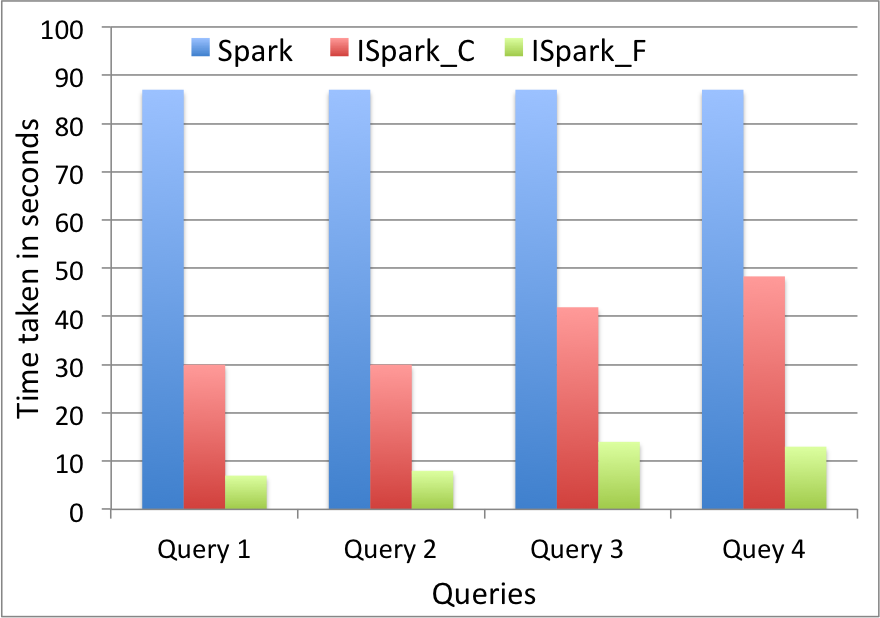
\includegraphics[scale=0.50]{./images/exp7.png}
\end{figure}

\paragraph{}
Fig. \ref{fig:exp8} shows a comparison of the three aforementioned
configurations when running the queries on 25GB file. The number of
partitions for ISpark\_C is 1,572, and that for ISpark\_F is 10,000.
While VSpark takes 220 seconds to complete, the average time for a
positive query using ISpark\_C is around 49 seconds. Using, more fine
grained partitioning ISpark\_F, the average time lowers down to 9
seconds. We can observe that while VSpark scales poorly as the size of % To be changed: Spark scales poorly
data increases, indexes helps the filtering query to scale in a more
scalable manner. With more fine grained partitioning, we were able to
reduce the overall query time for a 25GB over 10GB. However, limited by
the master node memory, we cannot further increase the number of
partitions. For future experiments, in order to scale up, we can
maintain a separate indexing server that can cache indexes and return
the set of RDDs on which a query has to be run. 

\begin{figure}[!ht]
\caption{Comparison of query completion times between Spark, Spark Coarse-grained and Spark Fine-grained partitioned for a 25GB file}
\label{fig:exp8}
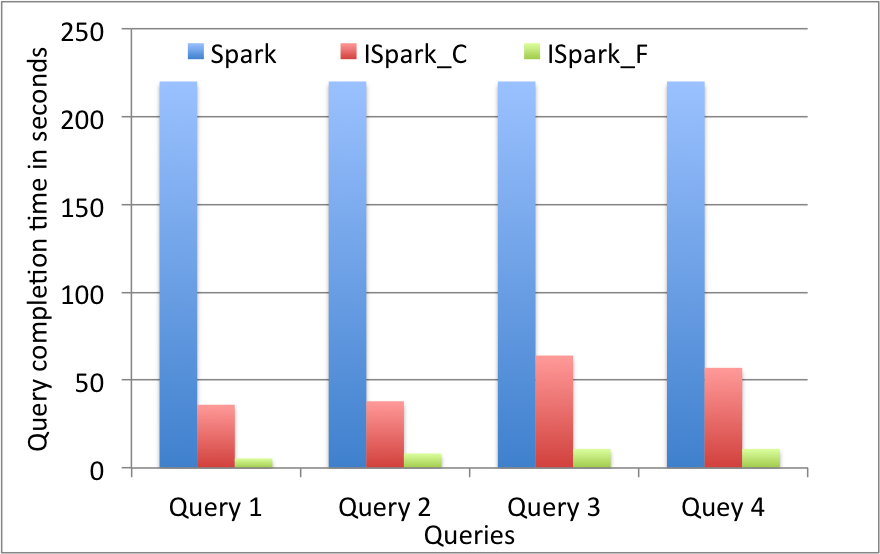
\includegraphics[scale=0.50]{./images/exp8.png}
\end{figure}

\paragraph{}
Fig. \ref{fig:exp9} shows the overall time it takes for the indexing
mechanism to initialize the partition metadata on the RDDs. The
partitioning schema scales in accordance with the filtering mechanisms
since the all the set of records have to be filtered. However, since
this is a one-time cost, the cost will be amortized with a batch of
queries. Besides, the time it takes to build indexes does not increase
by a large amount as the number of partitions increases. Therefore, fine
grained indexing can be very useful, as long the master has sufficient
memory to hold the index.

\begin{figure}[!ht]
\caption{Comparison of index creation time}
\label{fig:exp9}
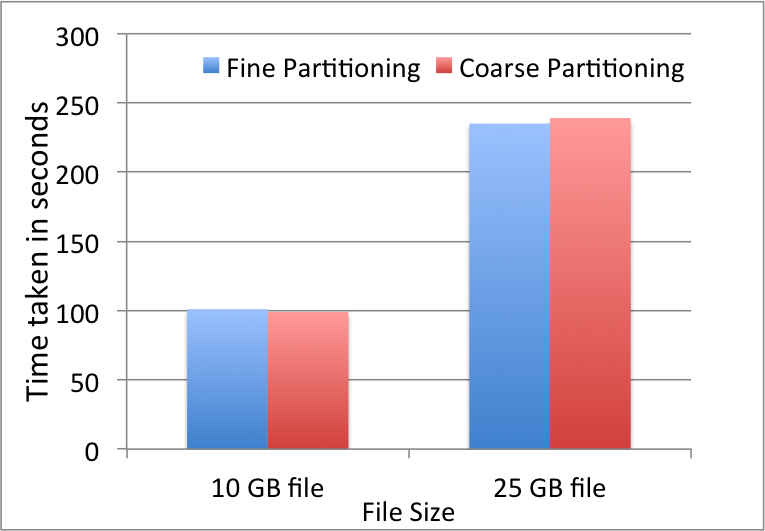
\includegraphics[scale=0.50]{./images/exp9.png}
\end{figure}

%\input{futurework}
\section{Related Work}
\label{sec:related}
\paragraph{}
We build our design on top of the Spark \cite{zaharia2012resilient}
runtime engine. While Spark provides useful abstractions for performing
distributed computations on top of RDDs, it lacks good support for
performing queries (such as \testtt{filter}, \texttt{count}, etc.) on
pre-specified keys.  Other frameworks such as Shark
\cite{engle2012shark}, Blink-DB \cite{agarwal2013blinkdb} have been used
for performing queries on top of Spark. However, they require data to be
completely structured as like data stored in RDBMS. We have designed our
system for semi-structured data, which consists of key-value pairs in
data files. 

\paragraph{}
Systems such as MANIMAL \cite{jahani2011automatic} perform automatic
optimizations on top of MapReduce programs. They can provide similar
optimizations by building B+ trees on data already stored within the
HDFS. However, our design works for an in-memory runtime engine, though
fundamentally it has some similar ideas.

\paragraph{}
Systems such as SSDAlloc\cite{badam2011ssdalloc} have looked at
detecting object-level accesses within native language programs. The
system relies on page protection mechanism which can be very expensive.
Our system intercepts object level accesses within a managed runtime and
is completely transparent, therefore addresses a different problem
subspace.

\section{Conclusion}
\label{sec:conclusion}
\paragraph{}
In the paper we presented detailed research on the impact of memory
pressure on the large in-memory computations. By quantifying the
detrimental impact of garbage collection on application runtime, we
provide useful insights into managing cluster level applications. We
posit that scaling horizontally by deploying more nodes with limited
memory may not scale applications as well as supporting individual nodes
with larger memory. We have also presented experiments and measured the
spectrum of object usage for a regular Spark application. We find that
the object access patterns are heavy-tailed and can be utilized to
manage memory better. Lastly, we explore further improvements in the
RDDs by building indexes on top of partitions, and show that we can
perform more efficient range queries with such design of Indexed RDDs.


%% Bibliography
%\vspace{-1ex}
%\linespread{1.0}
%\setlength{\bibsep}{1pt}
%\footnotesize
\small
\bibliography{local}
\bibliographystyle{abbrvnat}

\end{document}

